\chapter{Fundamentação teórica} \label{chap:fundamentacao}

Este capítulo visa realizar uma abordagem de toda a fundamentação teórica e tecnológica necessária para o entendimento da solução proposta neste trabalho.

\section{\mqtt}

O \textit{Message Queue Telemetry Transport} (\mqtt)\footnote{\url{http://mqtt.org}} é um protocolo baseado em mensagens e seguindo o modelo \pubsub, utiliza o conceito de tópicos gerenciados por componentes chamados de \brokers. Originalmente projetado para o uso em redes não confiáveis e com recursos limitados, consiste em um servidor \broker e dois tipos distintos de clientes, \pubs e \subs \cite{lee:et-al:2013}.

O \broker funciona como um intermediador entre as mensagens que são enviadas por \pubs e recebidas por \subs. Toda a comunicação é feita por intermédio de tópicos, que funcionam como uma hierarquia de diretórios onde as mensagens são entregues. Os \pubs publicam mensagens no \broker em um determinado tópico, e este se encarrega de realizar a entrega da mensagem para os \subs que registraram interesse naquele tópico, fazendo com que a orquestração da comunicação entre as entidades produtoras e consumidoras de dados seja feita exclusivamente pelo \broker. O processo de entrega de mensagens pode ser visto na \autoref{fig:mqtt-sequence}.

\begin{figure}[htb]
	\caption{Diagrama de sequência do processo de entrega de mensagens no \mqtt}
	\label{fig:mqtt-sequence}
	\centering
	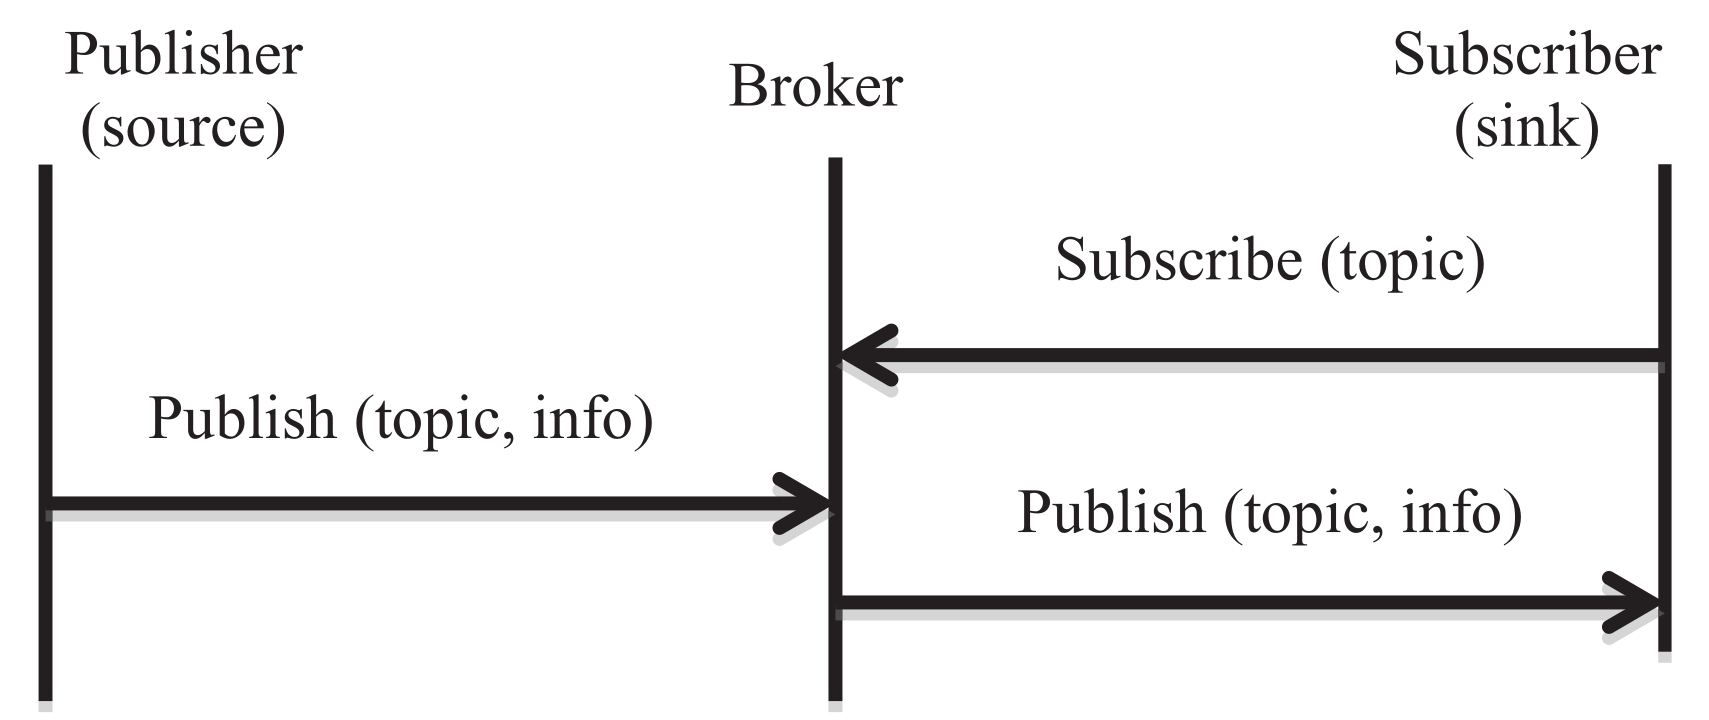
\includegraphics[width=0.85\linewidth]{img/mqtt-sequence.png}
	\fonte{\citeonline{al-fuqaha:et-al:2015}}
\end{figure}

Este protocolo permite o desacoplamento total entre os produtores e consumidores de dados, deste modo nenhum dos dois componentes têm ciência da existência mútua entre si.

\subsection{Tópicos \mqtt} \label{subsec:mqtt-topics}

Existem dois elementos em uma mensagem \mqtt---o dado e o tópico. O dado é a informação que o \pub precisa enviar, este dado será então enviado para o \sub que assinou o tópico onde a mensagem foi publicada \cite{tantitharanukul:et-al:2017}.

O \pub pode definir qualquer tópico para enviar uma mensagem, com um ou mais níveis de hierarquia, cada nível é separado por uma barra (e.g., \texttt{thailand/humidity} ou \texttt{thailand/bangkok/traffic}).

Também existe a conveniência da utilização de caracteres coringas para a assinatura de tópicos, como por exemplo \texttt{thailand/+/traffic} onde o caractere ``\texttt{+}'' corresponde a qualquer padrão de um único nível de uma hierarquia, neste caso terceiro nível, podendo ser utilizado para receber os dados de tráfego de qualquer cidade da Tailândia. Outro caractere coringa que pode ser utilizado é o ``\texttt{\#}'' que corresponde a todos os níveis subsequentes de uma hierarquia, este só pode ser utilizado como o último caractere de uma subscrição \cite{hunkeler:truong:stanford-clark:2008}.

Dado o seguinte tópico \texttt{a/b/c/d}, as seguintes assinaturas irão receber os dados publicados nele \cite{light:mosquitto}:

\begin{alineas}
	\item \texttt{a/b/c/d};
	\item \texttt{\#};
	\item \texttt{a/\#};
	\item \texttt{a/b/\#};
	\item \texttt{a/b/c/\#};
	\item \texttt{+/b/c/\#}.
\end{alineas}

O \mqtt é o protocolo padrão utilizado pelo \cddl para realizar troca de mensagens entre diferentes componentes, como será discutido na \autoref{subsec:cddl}.
		
\section{\mhubcddl}

O \mhubcddl é uma composição de um \gateway (\mhub) e um \middleware de \iomt (\cddl). Enquanto o \mhub transforma o dispositivo \android que está em execução em um \gateway \iot móvel responsável pela descoberta e aquisição de dados diretamente dos \smartobjs, o \cddl funciona como \middleware provendo serviços locais e remotos de descoberta de provedores de serviços, processamento de eventos complexos, publicação e assinatura de dados e eventos com qualidade de serviço.
A \autoref{fig:mhub-cdll-architecture} apresenta a arquitetura do \middleware.

\begin{figure}[htb]
	\centering
	\caption{\label{fig:mhub-cdll-architecture}Arquitetura do \mhubcddl}
	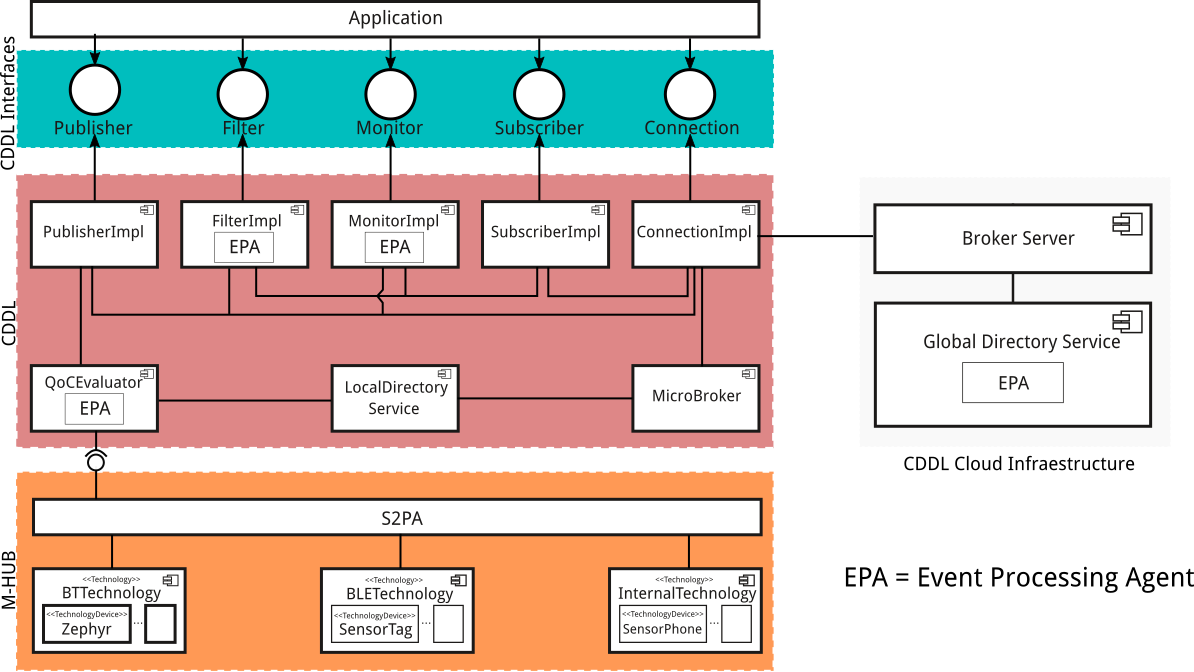
\includegraphics[width=0.85\linewidth]{img/mhub-cddl-architecture.png}
	\fonte{\citeonline[p.~15]{gomes:et-al:2017}}
\end{figure}

O \mhub faz o papel de \gateway móvel entre os \smartobjs e a Internet, onde os componentes mais inferiores encapsulam a heterogeneidade e especificidade das tecnologias WPAN suportadas.
O componente \texttt{BTTechnology} é voltado para a comunicação com dispositivos que utilizam a tecnologia \Bluetooth; a comunicação com \smartobjs que utilizam \Bluetooth \textit{Low Energy} é feita pelo componente \texttt{BLETechnology} enquanto a comunicação com sensores internos do dispositivo móvel é realizada por \texttt{InternalTechnology}.

O \stwopa é o serviço do \mhub que gerencia e oferece uma \api única para comunicação com as tecnologias suportadas.
Os dados coletados pelo \stwopa são pré-processados e enriquecidos com metadados de Qualidade de Informação (\textit{Quality of Information} -- QoI), e então encaminhados ao \cddl para distribuição.

O \qocevaluator é o componente do \cddl que recebe os dados adquiridos pelo \mhub.
Uma de suas responsabilidades é calcular dinamicamente o valor de alguns parâmetros de QoI que não puderam ser fornecidos na etapa de aquisição.
Após esta avaliação, esses parâmetros são adicionados como metadados aos dados de contexto que são encaminhados automaticamente ao \texttt{PublisherImpl}.

Todos os dados---oriundos do \stwopa ou providos pela camada de aplicação---são então publicados pelo \texttt{PublisherImpl} em uma estrutura de tópicos de um \broker \mqtt por intermédio do \texttt{ConnectionImpl}, componente que gerencia conexões e sessões das aplicações clientes com \brokers.
Desta forma os dados podem ser entregue às aplicações que registrarem, neste \broker, interesse em tais dados.

Também nota-se a presença de um componente chamado \texttt{MicroBroker}, este é uma versão reduzida do \broker \mqtt Moquette voltado para dispositivos \android\footnote{\url{https://github.com/technocreatives/moquette}}. Pode ser utilizado como alternativa a um \broker externo. Desta forma, os dados coletados ficam disponíveis apenas entre aplicações que executem no mesmo dispositivo.

\subsection{\mhub}

O \middleware \mhub pode ser definido, de acordo com \citeonline{talavera:et-al:2015}, como um serviço de \middleware de \iomt geral executado em um dispositivo móvel pessoal, responsável por descobrir e oportunisticamente conectar à uma miríade de \smartobjs acessíveis apenas através de tecnologias WPAN de curto alcance. Por estar envolvido com cenários de \iomt, este componente de \software tem que lidar com situações que apresentam muito mais indeterminismo, devido à fatores como a menor garantia de disponibilidade de sensores e atuadores, confiabilidade reduzida, maior volatilidade em conexões, etc.

O \smartphone executando uma instância do \mhub, funciona como \gateway para \smartobjs, fornecendo acesso à Internet para dispositivos que não podem se conectar. Outro recurso importante que pode ser explorado pelas aplicações é a habilidade de enriquecer os dados de sensores com dados de contexto obtidos dos sensores internos do \mhub.

Para que o \mhub tenha suporte à determinada tecnologia de comunicação, é necessário que um novo módulo seja implementado. Este módulo será responsável por gerenciar quaisquer operações que sejam necessárias para garantir o funcionamento desta tecnologia.

\subsubsection{\stwopa} \label{subsub:s2pa}

Para gerenciar a descoberta e conexão com dispositivos que trabalham com diferentes tecnologias de comunicação, além dos sensores internos do \smartphone, o \mhub utiliza o \textit{Short-range Sensing, Presence \& Actuation} (\stwopa), um protocolo que fornece uma \api comum para realizar a comunicação com diferentes tecnologias WPAN.

Implementado como um módulo na arquitetura do \middleware, o \stwopa define um conjunto de métodos e interfaces que os módulos responsáveis por determinada tecnologia de comunicação devem implementar. Isto permite que o \stwopa se comunique com todas as tecnologias WPAN suportadas, gerenciando-as, e assim fornece uma \api unificada para todas as camadas superiores da arquitetura que precisam se comunicar com tais tecnologias.

É possível encontrar na \autoref{fig:technology-interface} a interface \techinterface definida pelo \stwopa que declara os métodos padrões que realizam as funcionalidades básicas, a qual todas as tecnologias devem suportar.


\begin{figure}[htb]
	\centering
	\caption{\label{fig:technology-interface}Interface \techinterface}
	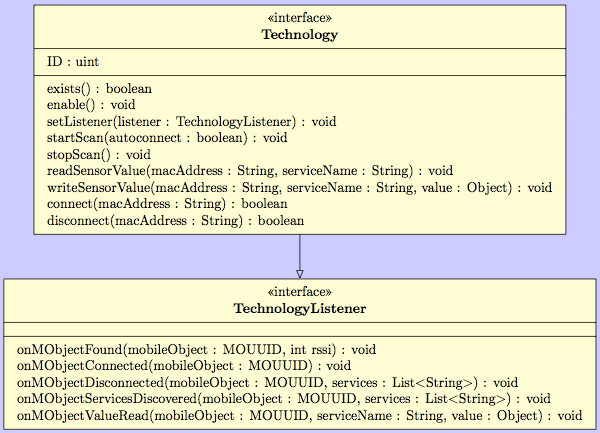
\includegraphics[width=0.85\linewidth]{img/technology-interface.png}
	\fonte{\citeonline[p.~125]{talavera:et-al:2015}}
\end{figure}

A interface \techinterface inclui inicialmente um identificador numérico \texttt{ID}, definido em tempo de programação, este define unicamente a tecnologia. Dentre os métodos métodos definidos pela interface, destaca-se:

\begin{alineas}
	\item \texttt{exists()}: Informa se o suporte à determinada tecnologia existe no dispositivo móvel onde o \middleware está executando;

	\item \texttt{enable()}: Habilita o uso da tecnologia para a aplicação;

	\item \texttt{startScan()}: Inicia o processo de escaneamento desta tecnologia. Recebe como parâmetro um valor booleano que indica se o componente responsável pela tecnologia deve tentar realizar o processo de conexão automaticamente ao encontrar um dispositivo durante o escaneamento;

	\item \texttt{stopScan()}: Finaliza o processo de escaneamento desta tecnologia;

	\item \texttt{connect()}: Recebe como parâmetro o endereço MAC de um \smartobj, e tenta realizar conexão com ele;

	\item \texttt{disconnect()}: Recebe um endereço MAC de um \smartobj como parâmetro, se conectado à ele, realiza a desconexão;

	\item \texttt{readSensorValue()}: Recebe como parâmetro o endereço MAC e o nome de um serviço fornecido por um \smartobj e realiza o processo de leitura de dados fornecido por aquele serviço.
\end{alineas}

Outro método importante é o \texttt{setListener()}, que recebe como parâmetro uma instância de uma classe que implemente a interface \techlistener, também apresentada na \autoref{fig:technology-interface}.
Todas as informações relevantes sobre \smartobjs descobertos pelas tecnologias geram eventos, estes são capturados através de \techlistener.
Esta interface define métodos que serão acionados de acordo com o acontecimento de certos eventos por parte de alguma tecnologia de comunicação.
Dentre os métodos, tem-se:

\begin{alineas}
	\item \texttt{onMobjectFound()}: Executado quando uma tecnologia encontra um \smartobj;

	\item \texttt{onMobjectConnected()}: Executado quando uma tecnologia se conecta à um \smartobj;

	\item \texttt{onMobjectDisconnected()}: Executado quando uma tecnologia se desconecta à um \smartobj;

	\item \texttt{onMobjectValueRead()}: Executado quando uma tecnologia realiza uma leitura por parte de um \smartobj;
\end{alineas}

O \stwopa é uma classe que implementa a interface \techlistener.
Ela é responsável por iniciar cada tecnologia e se cadastrar através do método \texttt{setListener()} como o \listener daquela tecnologia.
As tecnologias se comunicam com o \stwopa através dos métodos de \techlistener descritos acima, desta forma o \stwopa recebe todas a interações com os \smartobjs, implementando assim o padrão de projeto \textit{observer}~\cite{gamma:et-al:1994}.

Quando o \stwopa recebe de alguma tecnologia, um evento de descoberta, conexão, desconexão ou leitura de dados de \smartobjs, ele o encapsula em um objeto do tipo \sensordata.
Esta classe possui os seguintes atributos:

\begin{alineas}
	\item \texttt{mouuid}: Uma combinação entre o \textit{id} da tecnologia que gerou tal evento com o endereço MAC do \smartobj;

	\item \texttt{signal}: Número em ponto flutuante onde o RSSI (\textit{Receiver Signal Strength}) daquela interação com o \smartobj é armazenado. O RSSI representa a intensidade de sinal naquele momento;

	\item \texttt{action}: Indica que tipo de evento uma instância de \sensordata está encapsulando. Os valores possíveis são as constantes:

	\begin{alineas}

		\item \texttt{FOUND}: Indica que um \smartobj foi descoberto pelo \mhub no ambiente;

		\item \texttt{CONNECTED}: Indica que o \mhub realizou uma conexão com o \smartobj;

		\item \texttt{READ}: Indica que uma leitura foi realizada, ou seja, o \smartobj enviou dados ao \mhub;

		\item \texttt{DISCONNECTED}: Indica que a conexão com o \smartobj foi desfeita.

	\end{alineas}

	\item \texttt{sensorName}: Representa o nome do \smartobj;

	\item \texttt{sensorValue}: Um vetor de pontos flutuantes que armazena os valores lidos do \smartobj. Logicamente este atributo só possui valores quando o atributo \texttt{action} assume o valor \texttt{READ}.
\end{alineas}

Os objetos do tipo \sensordata gerados no \stwopa a partir de leitura de dados de \smartobjs são enviados para o \cddl para distribuição.

O \mhub fornece diversos serviços que não serão tratados neste trabalho, dentre eles, destaca-se \cite{gomes:2017}:

\begin{alineas}
	\item \emph{protocolo de transcodificação}:
		Os pacotes de dados recebidos dos sensores podem ter diferentes formatos e codificações.  Assim, o \mhub deve transcodificá-los e serializá-los, antes de transmiti-los. A transcodificação de dados é altamente dependente do tipo, marca e fabricante do sensor;
		
	\item \emph{caching de dados}:
		A fim de otimizar a transmissão para a nuvem através da Internet móvel, o \mhub pode agrupar várias amostras de dados obtidas a partir de vários sensores próximos antes de enviá-las ao \gateway em rajada única. Para isso, o \mhub armazena em cache as amostras de dados recebidas dos sensores;
		
	\item \emph{configuração e controle dos sensores}:
		Dependendo do tipo de sensor, o \mhub pode, eventualmente ou periodicamente, enviar comandos, definições de parâmetros ou requisições de consultas de dados através da WPAN para os sensores conectados;
		
	\item \emph{pré-processamento de dados do sensor}:
		Antes de enviar os dados, pode ser necessário aplicar uma função de pré-processamento (e.g.  transcodificação, formatação, agregação, filtragem, ou comparação com leituras anteriores etc.).  Esse pré-processamento é feito no \mhub;
		
	\item \emph{carregamento dinâmico de módulos do sensor}:
		Uma vez que não é possível ter módulos internos para todos os sensores que podem estar disponíveis a medida que o \gateway se move, o \mhub oferece um mecanismo de implantação de módulo em tempo de execução e gerenciamento do ciclo de vida desses módulos;
		
	\item \emph{processamento nas pontas}:
		O \mhub oferece mecanismos que permitem aos desenvolvedores de aplicações distribuírem as funcionalidades do seu código entre o dispositivo móvel e nodos da nuvem, movendo parte do processamento das informações de contexto para “as pontas” do sistema. A isso se dá o nome de In-Network Processing, uma técnica que ajuda a diminuir a quantidade de informações a ser transmitida para a nuvem, podendo melhorar a escalabilidade do sistema. O processamento ao qual esta funcionalidade se refere pode ser implementado em código Java convencional ou utilizando EPL Esper;
		
	\item \emph{processamento ciente de energia}:
		Por meio de um componente de gerenciamento de energia, o \mhub monitora o nível da bateria do dispositivo móvel, disparando ações adaptativas que ajustam os comportamento dos seus serviços, de acordo com a disponibilidade de energia do dispositivo móvel. Por exemplo, a frequência de publicação dos dados por ser reduzida quando o nível da bateria está baixo (por exemplo, menor que 20\%).
\end{alineas}

\subsection{\cddl} \label{subsec:cddl}

O \cddl é uma camada de distribuição de dados que provê mecanismos que permitem a especificação, controle e monitoramento de requisitos de qualidade de informação e do serviço de distribuição de dados \cite{gomes:2017}.

Como \middleware, o \cddl permite que as aplicações clientes assumam o papel de produtoras ou consumidoras de dados de contexto, fornecendo suporte à políticas de qualidade de serviço de distribuição de dados. Desta forma as aplicações podem especificar parâmetros que expressam seus requisitos de QoC para envio e recebimento de mensagens. A fim de fornecer suporte para o desenvolvimento de aplicações de \iot e \iomt, o \cddl atende aos seguintes requisitos \cite{muniz:2017}:

\begin{alineas}
	\item suporte à distribuição de dados local e remota;

	\item suporte ao registro e descoberta distribuída de serviços;

	\item modelo de programação uniforme e independente de localização;

	\item suporte à entrega confiável de dados em cenários de mobilidade;

	\item provisionamento e monitoramento de qualidade da informação;

	\item provisionamento e monitoramento de qualidade do serviço de distribuição;

	\item filtragem das informações.
\end{alineas}

A interação entre produtores e consumidores de dados de contexto se dá através do modelo \pubsub com a utilização de \brokers, implementando uma comunicação distribuída com o \mqtt. O \cddl também fornece um \ubroker que executa internamente no dispositivo móvel, o que permite que certas aplicações possam publicar e receber dados sem a dependência de conexão à Internet.

O \cddl recebe através de \eventbus objetos do tipo \sensordata vindos do \stwopa.
Este objeto é convertido em um objeto do tipo \msg, todos os dados publicados pelo \cddl são instâncias desta classe.
Este novo objeto é então anotado com alguns parâmetros de QoI que não puderam ser informados no momento de captura do dado.
Esta classe encapsula diversos atributos relevantes aos dados de contexto que representam, dentre eles, destaca-se:

\begin{alineas}
	\item \texttt{serviceName}: Nome do \smartobj que está relacionado a essa \msg;

	\item \texttt{serviceValue}: Valor da leitura dos dados do \smartobj;

	\item \texttt{accuracy}: Acurácia do dado;

	\item \texttt{measurementTime}: O \timestamp em que a \msg foi gerada;

	\item \texttt{sourceLocationLatitude}: Latitude do \mhub que gerou este dado;

	\item \texttt{sourceLocationLongitude}: Longitude do \mhub que gerou este dado;

	\item \texttt{sourceLocationAltitude}: Altitude do \mhub que gerou este dado;

	\item \texttt{signal}: Intensidade do sinal no momento em que o \smartobj interagiu com o \stwopa.
\end{alineas}

Ao receber um dado de contexto vindo do \stwopa, o \cddl automaticamente o serializa em formato JSON e o publica em um \broker \mqtt definido no momento da inicialização do \middleware. 
O atributo \texttt{serviceName} é utilizado para gerar parte do tópico.

A \autoref{fig:general-vision-cddl} ilustra o uso da infraestrutura \mhubcddl em um cenário de \textit{Ambient Assisted Living}. Neste cenário os pacientes têm seus dados vitais monitorados por uma rede de sensores corporais.
Os dados são coletados por \smartphones equipados com aplicações \mhubcddl que distribuem os dados em um conjunto de \brokers em nuvem.  
Estes dados podem ser entregues aos médicos ou cuidadores e familiares do paciente.

\begin{figure}[htb]
	\centering
	\caption{Visão geral do \mhubcddl em um cenário de \iomt}
	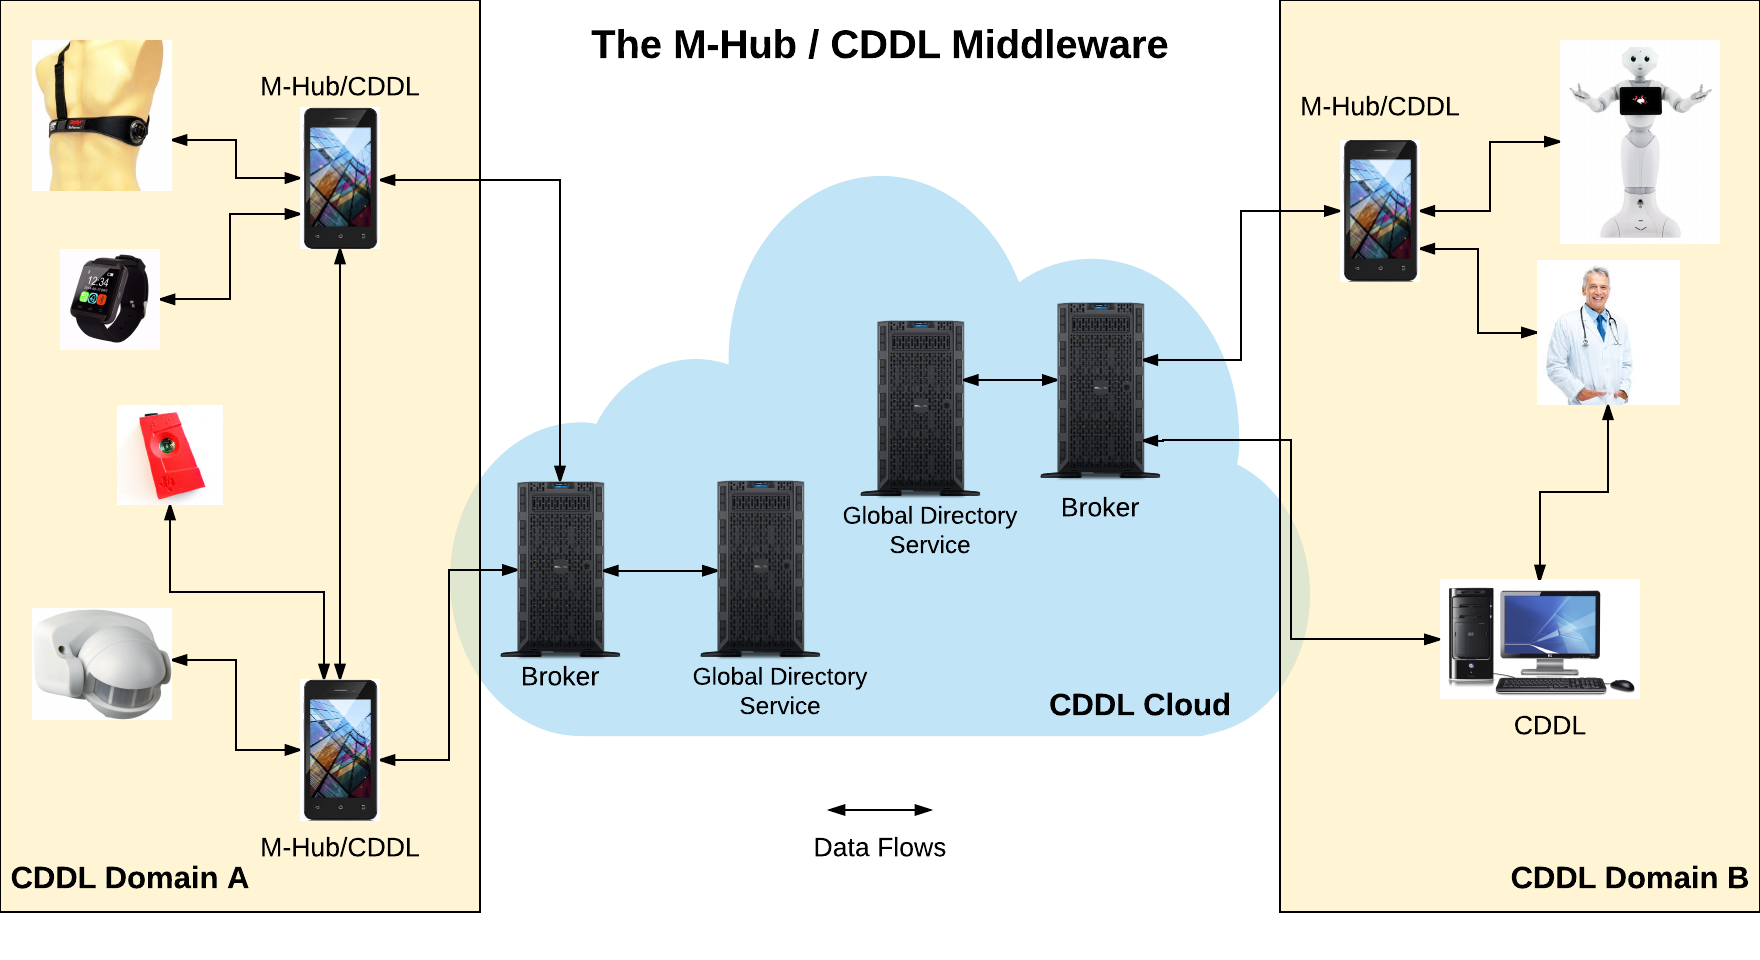
\includegraphics[width=.85\linewidth]{img/general-vision-cddl.png}
	\fonte{\citeonline{gomes:et-al:2017}}
	\label{fig:general-vision-cddl}
\end{figure}

%\subsubsection{Modelo de programação}

Como já mencionado, o modelo de programação do \cddl respeita o padrão \pubsub, o \middleware oferece então duas classes: \texttt{Publisher} e \texttt{Subscriber} para realizar publicações e inscrições em tópicos, respectivamente.
Uma aplicação que registra o interesse por algum tipo de dado de contexto será notificada através de um objeto \msg, que representa este dado.
O \autoref{lst:subscriber} apresenta um exemplo de como o desenvolvedor pode consumir dados de temperatura capturados pelo \middleware.

\lstinputlisting[float=htb,label=lst:subscriber, caption=Modelo de programação \pubsub do \cddl]{code/Subscriber.java}

Nas linhas 1 e 2, uma instância de \texttt{Subscriber} é criada e uma conexão com um \broker é feita.
Na linha 3 o programa registra interesse em dados do serviço de temperatura, internamente o \texttt{Subscriber} irá se inscrever em um tópico onde todos os dados de contexto deste serviço são publicados.
Nas linhas 5 até 13 um \textit{listener} para este objeto é definido, é a partir deste que os dados serão capturados.
Todos os dados de contexto provenientes do serviço temperatura, chegarão ao método \texttt{onMessageArrived} como uma instância de \msg.

